% Workshop draft — §5.1. Independent of intro / §5.2 wording.
% Numbers: output/panocrowd/metrics.json (PanoCrowd val∪test).
% Do not rewrite this as the body-column experiment. k=48 is not the claim.

\section{Spherical Seams Already Miss Most Two-Degree Heads}
\label{sec:head-disks}

Class-weighted energy is the obvious semantic correction: raise the cost
of people so seams take corridors. Outdoor stills (CVRG-Pano) did not
supply that test. People there are rare and already high-gradient;
$(c)-(b)$ person overlap was $\approx 0$, and a screen of val$\cup$test
plus train found no low-texture foreground people. PanoCrowd is the
content condition that should break the redundancy: heads are the scene,
and ground-truth points give disks that can be both the energy and the
metric. This section is that experiment. It is not a person-damage
null, and it is not the body-column follow-up of~\S\ref{sec:body-boundary}.

\paragraph{Protocol.}
Official val$\cup$test ($n=313$), not train. Density bins follow the
dataset's own counts: sparse $0$--$49$ heads ($n=72$), medium $50$--$199$
($n=171$; the claim bin), dense $200+$ ($n=70$). Both configs use cyclic
$8$-connected DP, $24$ seams at width $\le 512$, $\lambda_g=\lambda_p=1$.
Config (b) is gradient$\times\cos\phi$ only ($\lambda_s=0$). Config (c)
adds semantic energy ($\lambda_s=4$) from GT head points painted as
latitude-aware $2^\circ$ disks: equatorial radius $W\times(2^\circ/360)$,
$r(\phi)=r_{\mathrm{eq}}/\max(|\cos\phi|,\cos 75^\circ)$. A head is hit
if any of the first $k$ original-width seams, on that head's row, has
cyclic $|x-x_{\mathrm{head}}|\le r(\phi)$. Energy disks use the same
$r(\phi)$, so the term protects what the test scores. Primary $k=24$.
We also record $k\in\{8,48\}$; $k=48$ is not the claim.

\paragraph{Locked bar.}
Support on medium, $k=24$, requires a mean reduction of at least $5$\,pp
\emph{and} a majority of images with (c)$<$(b). Characterized-boundary
further requires sparse $\Delta$ strictly weaker than medium. The bar
was not moved after seeing the table.

\begin{table}[t]
\centering
\caption{Head-hit rate, GT $2^\circ$ disks, $k=24$. Equatorial disk
cover is a flattening diagnostic, not an outcome. Body-column rates
are a separate experiment (\S\ref{sec:body-boundary}) and are not in
this table.}
\label{tab:head-disks}
\begin{tabular}{lrrrrrr}
\toprule
Bin & $n$ & hit (b) & hit (c) & $\Delta$ & (c)$<$(b) & eq cover \\
\midrule
Sparse $0$--$49$ & $72$ & $4.5\%$ & $0.1\%$ & $-4.39$\,pp & $26/72$ & $0.8\%$ \\
Medium $50$--$199$ & $171$ & $4.3\%$ & $0.1\%$ & $-4.18$\,pp & $82/171$ & $2.2\%$ \\
Dense $200+$ & $70$ & $3.7\%$ & $0.0\%$ & $-3.64$\,pp & $31/70$ & $5.3\%$ \\
\bottomrule
\end{tabular}
\end{table}

\paragraph{Verdict: dense-null.}
Medium $\Delta$ is $-4.18$\,pp, not $\le -5$. Majority is $82/171$
($48\%$), not a majority. Sparse $\Delta$ is slightly \emph{larger}
than medium ($-4.39$ vs.\ $-4.18$), so a density-conditioned thesis
would have failed even if the $5$\,pp had landed. The stress bin is
populated ($n=171$); this is a real miss against the locked bar, not
an empty regime.

\paragraph{The ceiling is $4.3$\,pp.}
Medium (b) hits only $4.3\%$ of heads. If (c) hits none, the most
negative mean $\Delta$ available is $-4.3$\,pp. Observed $-4.18$\,pp
uses essentially that whole range: (c) is never worse than (b) at
$k=24$ ($0/313$ images). The near-miss is a low baseline, not a
failure of the semantic term to mop what little (b) still hits. That
explains why the bar was almost unavailable. It does not rewrite the
bar, and it does not license calling $2^\circ$ hits a settled
person-damage null: the metric is a small disk on a head point.

At $k=8$ the medium reduction is $-1.65$\,pp ($56/171$). At $k=48$ it
is $-8.73$\,pp ($120/171$), which would have met the $5$\,pp bar. The
spec said that if only $k=48$ meets it, that is a robustness note, not
the result. We do not promote $k=48$.

\paragraph{Exploratory only.}
Among the $84$ medium images where (b) hits at least one head, $82/84$
go down and the mean $\Delta$ is $-8.5$\,pp. The other $87$ are $0\to 0$
ties (thin seams versus clustered $2^\circ$ disks). Report that as a
hypothesis about a low baseline hit rate, not as the result.

\begin{figure}[t]
  \centering
  \begin{minipage}[t]{0.48\linewidth}
    \centering
    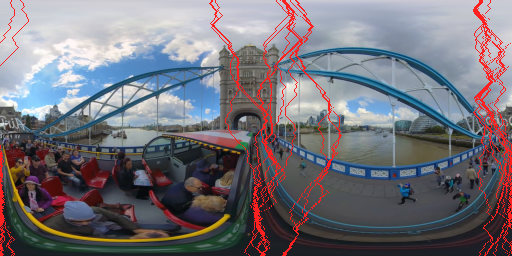
\includegraphics[width=\linewidth]{figures/fig_head_max_b.png}\\
    {\small (b) spherical, largest medium $\Delta$}
  \end{minipage}\hfill
  \begin{minipage}[t]{0.48\linewidth}
    \centering
    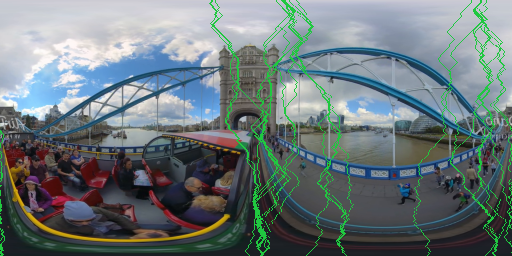
\includegraphics[width=\linewidth]{figures/fig_head_max_c.png}\\
    {\small (c) $2^\circ$ head-disk energy}
  \end{minipage}
  \caption{Largest medium-bin head-hit reduction, not a typical image
  ($87/171$ medium frames are $0\to 0$ at $k=24$). Red: (b) seams.
  Green: (c) seams. Even here the work is mopping a remainder: (b)
  already misses most $2^\circ$ heads.}
  \label{fig:head-max}
\end{figure}

\paragraph{What this does and does not show.}
Gradient$\times\cos\phi$ already misses most $2^\circ$ heads in every
density bin, including the stress bin. Semantic energy uses nearly
the entire available ceiling and still misses a bar that assumed more
head-cutting to undo. That is a finding about this metric, not a
finding that seams do not cut people. Scoring the same (b) seams
against a $12^\circ$ body-column proxy later put the medium baseline
at $12.6\%$, inside a pre-registered $[10\%,20\%)$ do-not-settle
interval. Body-column energy versus spherical energy was then locked
as its own experiment (\S\ref{sec:body-boundary}). It was not the
original plan, and it does not rewrite the table above.
